%%%%%%%%%%%%%%%%%%%%%%%%%%%%%%%%%%%%%%%%%
% Programming/Coding Assignment
% LaTeX Template
%
% This template has been downloaded from:
% http://www.latextemplates.com
%
% Original author:
% Ted Pavlic (http://www.tedpavlic.com)
%
% Note:
% The \lipsum[#] commands throughout this template generate dummy text
% to fill the template out. These commands should all be removed when 
% writing assignment content.
%
% This template uses a Perl script as an example snippet of code, most other
% languages are also usable. Configure them in the "CODE INCLUSION 
% CONFIGURATION" section.
%
%%%%%%%%%%%%%%%%%%%%%%%%%%%%%%%%%%%%%%%%%

%----------------------------------------------------------------------------------------
%	PACKAGES AND OTHER DOCUMENT CONFIGURATIONS
%----------------------------------------------------------------------------------------

\documentclass{article}

\usepackage{fancyhdr} % Required for custom headers
\usepackage{lastpage} % Required to determine the last page for the footer
\usepackage{extramarks} % Required for headers and footers
\usepackage[usenames,dvipsnames]{color} % Required for custom colors
\usepackage{graphicx} % Required to insert images
\usepackage{listings} % Required for insertion of code
\usepackage{courier} % Required for the courier font
\usepackage{lipsum} % Used for inserting dummy 'Lorem ipsum' text into the template

% Margins
\topmargin=-0.45in
\evensidemargin=0in
\oddsidemargin=0in
\textwidth=6.5in
\textheight=9.0in
\headsep=0.25in

\linespread{1.1} % Line spacing

% Set up the header and footer
\pagestyle{fancy}
\lhead{\hmwkAuthorName} % Top left header
\chead{\hmwkClass\ (\hmwkClassInstructor\ \hmwkClassTime): \hmwkTitle} % Top center head
\rhead{\firstxmark} % Top right header
\lfoot{\lastxmark} % Bottom left footer
\cfoot{} % Bottom center footer
\rfoot{Page\ \thepage\ of\ \protect\pageref{LastPage}} % Bottom right footer
\renewcommand\headrulewidth{0.4pt} % Size of the header rule
\renewcommand\footrulewidth{0.4pt} % Size of the footer rule

\setlength\parindent{0pt} % Removes all indentation from paragraphs

%----------------------------------------------------------------------------------------
%	CODE INCLUSION CONFIGURATION
%----------------------------------------------------------------------------------------

\definecolor{MyDarkGreen}{rgb}{0.0,0.4,0.0} % This is the color used for comments
\lstloadlanguages{Perl} % Load Perl syntax for listings, for a list of other languages supported see: ftp://ftp.tex.ac.uk/tex-archive/macros/latex/contrib/listings/listings.pdf
\lstset{language=Perl, % Use Perl in this example
        frame=single, % Single frame around code
        basicstyle=\small\ttfamily, % Use small true type font
        keywordstyle=[1]\color{Blue}\bf, % Perl functions bold and blue
        keywordstyle=[2]\color{Purple}, % Perl function arguments purple
        keywordstyle=[3]\color{Blue}\underbar, % Custom functions underlined and blue
        identifierstyle=, % Nothing special about identifiers                                         
        commentstyle=\usefont{T1}{pcr}{m}{sl}\color{MyDarkGreen}\small, % Comments small dark green courier font
        stringstyle=\color{Purple}, % Strings are purple
        showstringspaces=false, % Don't put marks in string spaces
        tabsize=5, % 5 spaces per tab
        %
        % Put standard Perl functions not included in the default language here
        morekeywords={rand},
        %
        % Put Perl function parameters here
        morekeywords=[2]{on, off, interp},
        %
        % Put user defined functions here
        morekeywords=[3]{test},
       	%
        morecomment=[l][\color{Blue}]{...}, % Line continuation (...) like blue comment
        numbers=left, % Line numbers on left
        firstnumber=1, % Line numbers start with line 1
        numberstyle=\tiny\color{Blue}, % Line numbers are blue and small
        stepnumber=5 % Line numbers go in steps of 5
}

% Creates a new command to include a perl script, the first parameter is the filename of the script (without .pl), the second parameter is the caption
\newcommand{\perlscript}[2]{
\begin{itemize}
\item[]\lstinputlisting[caption=#2,label=#1]{#1.pl}
\end{itemize}
}

%----------------------------------------------------------------------------------------
%	DOCUMENT STRUCTURE COMMANDS
%	Skip this unless you know what you're doing
%----------------------------------------------------------------------------------------

% Header and footer for when a page split occurs within a problem environment
\newcommand{\enterProblemHeader}[1]{
\nobreak\extramarks{#1}{#1 continued on next page\ldots}\nobreak
\nobreak\extramarks{#1 (continued)}{#1 continued on next page\ldots}\nobreak
}

% Header and footer for when a page split occurs between problem environments
\newcommand{\exitProblemHeader}[1]{
\nobreak\extramarks{#1 (continued)}{#1 continued on next page\ldots}\nobreak
\nobreak\extramarks{#1}{}\nobreak
}

\setcounter{secnumdepth}{0} % Removes default section numbers
\newcounter{homeworkProblemCounter} % Creates a counter to keep track of the number of problems

\newcommand{\homeworkProblemName}{}
\newenvironment{homeworkProblem}[1][Problem \arabic{homeworkProblemCounter}]{ % Makes a new environment called homeworkProblem which takes 1 argument (custom name) but the default is "Problem #"
\stepcounter{homeworkProblemCounter} % Increase counter for number of problems
\renewcommand{\homeworkProblemName}{#1} % Assign \homeworkProblemName the name of the problem
\section{\homeworkProblemName} % Make a section in the document with the custom problem count
\enterProblemHeader{\homeworkProblemName} % Header and footer within the environment
}{
\exitProblemHeader{\homeworkProblemName} % Header and footer after the environment
}

\newcommand{\problemAnswer}[1]{ % Defines the problem answer command with the content as the only argument
\noindent\framebox[\columnwidth][c]{\begin{minipage}{0.98\columnwidth}#1\end{minipage}} % Makes the box around the problem answer and puts the content inside
}

\newcommand{\homeworkSectionName}{}
\newenvironment{homeworkSection}[1]{ % New environment for sections within homework problems, takes 1 argument - the name of the section
\renewcommand{\homeworkSectionName}{#1} % Assign \homeworkSectionName to the name of the section from the environment argument
\subsection{\homeworkSectionName} % Make a subsection with the custom name of the subsection
\enterProblemHeader{\homeworkProblemName\ [\homeworkSectionName]} % Header and footer within the environment
}{
\enterProblemHeader{\homeworkProblemName} % Header and footer after the environment
}

%----------------------------------------------------------------------------------------
%	NAME AND CLASS SECTION
%----------------------------------------------------------------------------------------

\newcommand{\hmwkTitle}{FE - Assignment\ \#05} % Assignment title
\newcommand{\hmwkDueDate}{Friday,\ February\ 19,\ 2016} % Due date
\newcommand{\hmwkClass}{MA\ 374} % Course/class
\newcommand{\hmwkClassTime}{} % Class/lecture time
\newcommand{\hmwkClassInstructor}{} % Teacher/lecturer
\newcommand{\hmwkAuthorName}{Silvi Pandey(130123045)} % Your name

%----------------------------------------------------------------------------------------
%	TITLE PAGE
%----------------------------------------------------------------------------------------

\title{
\vspace{2in}
\textmd{\textbf{\hmwkClass:\ \hmwkTitle}}\\
\normalsize\vspace{0.1in}\small{Due\ on\ \hmwkDueDate}\\
\vspace{0.1in}\large{\textit{\hmwkClassInstructor\ \hmwkClassTime}}
\vspace{3in}
}

\author{\textbf{\hmwkAuthorName}}
\date{} % Insert date here if you want it to appear below your name

%----------------------------------------------------------------------------------------

\begin{document}

\maketitle

%----------------------------------------------------------------------------------------
%	TABLE OF CONTENTS
%----------------------------------------------------------------------------------------

%\setcounter{tocdepth}{1} % Uncomment this line if you don't want subsections listed in the ToC

\newpage


%----------------------------------------------------------------------------------------
%	PROBLEM 1
%----------------------------------------------------------------------------------------

% To have just one problem per page, simply put a \clearpage after each problem
\begin{center}
\textbf{PROBLEM - 1}
\end{center}
Consider the same data given in Lab 04 (Problem 1) to construct the efficient frontier. Now, construct the
minimum variance curve (and efficient frontier) and the feasible region (in the risk-return plot) assuming that
short sales are not allowed. In the same plot, also indicate the minimum variance curves (there are three of those)
if you consider any two out of three securities at a time. Also, in another graph, plot the weights corresponding
to the minimum variance curve (and write the equation that these weights satisfy).
\begin{center}
\textbf{SOLUTION}
\end{center}
The weights corresponding to the minimum variance portfolio can be obtained by minimising the variance subject to the constraint that the sum of the respective weights is equal to 1 . The following is the expression for the weights corresponding to the minimum variance portfolio. :
\begin{center}
\includegraphics{Formula}
\end{center}
\textbf{Without short sell}
\begin{center}
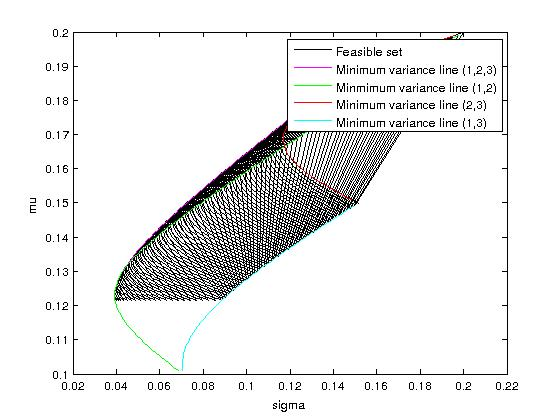
\includegraphics[width=80mm]{WithoutShortSell}
\end{center}

\textbf{With short sell}
\begin{center}
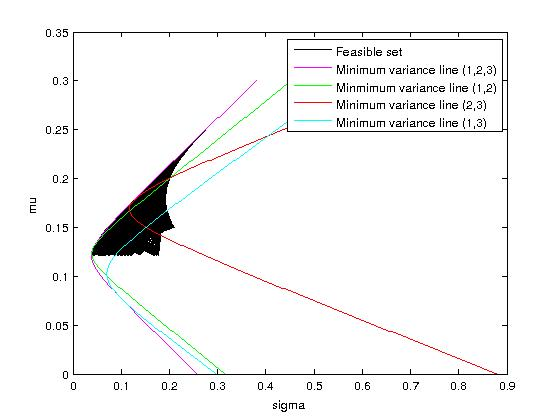
\includegraphics[width=80mm]{WithShortSell}
\end{center}

In the plot corresponding to 'Without short sell' the weights are forced to be positive while this restriction is not there in the plot corresponding to 'With short sell'. As observed from the plot,when short sell is not allowed, the efficient frontier is just the part above the minimum variance portfolio while the efficient frontier covers the entire minimum variance line in the case where short sell is allowed
\newpage
\textbf{Weights corresponding to the minimum variance line}
\begin{center}
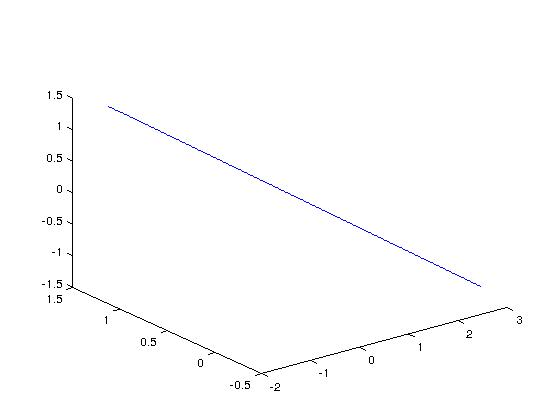
\includegraphics[width=100mm]{w1_w2_w3}.
\end{center}

The above is a line plot in three dimensions satisfying the equation $w_{1}+w_{2}+w_{3} = 1$ and belonging to the minimum variance line.As expected the  plot is a plane in 3D.

\begin{center}
\textbf{PROBLEM - 2}
\end{center}
Recall the Lab 04 assignment with the data part (Problem 2). In a similar way, do the following: Collect the
data of basic BSE and NSE index values (from their respective official websites) for the period from January
1, 2007 to December 31, 2015. Now, for the same period, collect the stock price data for 10 stocks that are
included in the index and 10 stocks that are not included in the index, for each of the index. Repeat what you
have done in Lab 04, with the index as market portfolio (for both the indices). From the CAPM formula (SML),
draw inference about each of the stocks. Try to compare the betas of securities (by taking the actual data and
computing from your data for each index).
Keep the data in two separate Excel files and name them as “bsedata1” and “nsedata1”. Obtain data on stocks
yourself and do not copy from others. We will use these data in future assignments too.

\begin{center}
\textbf{SOLUTION}
\end{center}

\textbf{From BSE (SP-BSE100):}\\
The index chosen was SP-BSE 100 and it included around 80-100 stocks.Out of which 10 stocks were chosen and 10 stocks which were not a part of the index was also chosen.\\
The following 10 stocks were taken from BSE index : ABB-India ltd , ACC ltd, Adani Ports and Special Economic Zone, Ambuja Cements ltd, Ashok Leyland ltd , Asian Paints ltd, Aurobindo Pharma ltd , Axis Bank ltd, Bank Of Baroda , Bank Of India.\\
The following 10 stocks were taken which aren't part of BSE index : Aditya Birla Nuvo ltd, Alphabet ltd, Amazon ltd, Dadone ltd, Dollar General Corporation, Facebook ltd , Hess Corporation , Liberty Lilac Group ,MTNL , Taj Hotels.\\\\

In part 1 of the problem, the beta values for every stock was calculated using the index as the market portfolio. Firstly, the return of one of the stock was plotted against the market portfolio.In order to calculate the beta values the returns ($K_{v} , K_{m}$) were fit in a line using regression.The following is the expression for beta :
$$\beta = \frac{Cov(K_{v},K_{m})}{\sigma_{m}^{2}}$$
The following scatter plot was obtained between the return of 'Aditya Birla Nova Ltd' and the market portfolio formed from the BSE index. 
\begin{center}
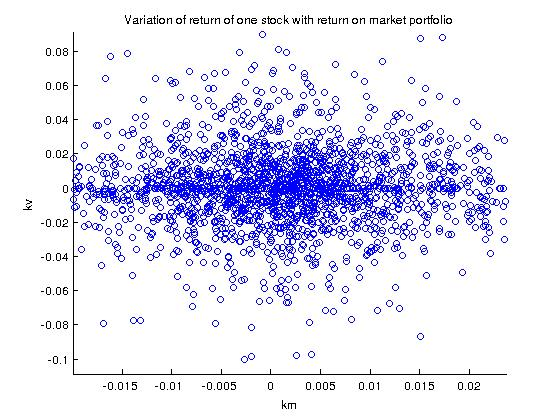
\includegraphics[width=100mm]{scatterPlotAdityaBirlaNuvoLtd}
\end{center}
The $\beta$ values for the stocks not included in the index are (in the order as mentioned above) :\\
\begin{center}
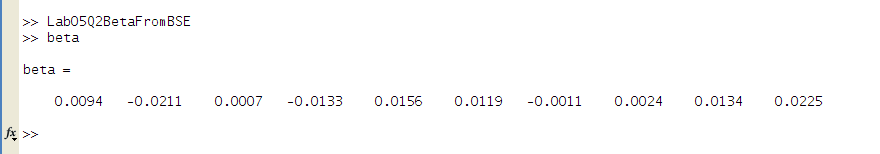
\includegraphics[width=100mm]{BetaBSE}
\end{center}
The $\beta$ values of the stocks included in the index are (in the order as mentioned above) :\\
\begin{center}
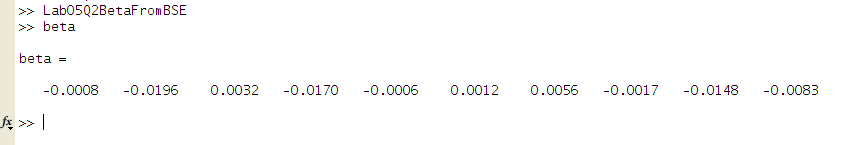
\includegraphics[width=100mm]{BetaStocksIncludedBSE}
\end{center}
Now, the stocks included in the index was used to simulate the index (market portfolio) by taking the weighted average of the prices of the stocks and doing a similar exercise.

The $\beta$ values of the stocks not included in the index obtained by simulating the index from the ten stocks already in the BSE index are (in the order as mentioned above ):\\
\begin{center}
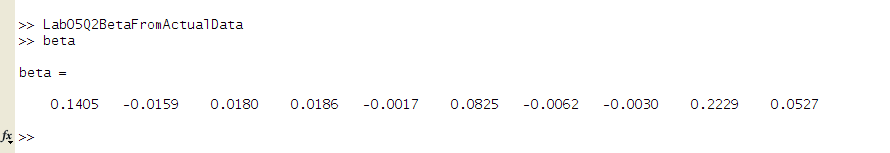
\includegraphics[width=100mm]{BetaActualDataBSE}
\end{center}

\newpage
\textbf{From NSE (NIFTY 100):}\\
The following 10 stocks were taken from NSE index : ACC ltd, Adani Ports and Special Economic Zone, Ambuja Cements ltd, Apollo Hospital , Asian Paints, Aurobindo Pharma ltd, Axis Bank ltd, Bank Of Baroda, Bank Of India, Bosch ltd\\
The following 10 stocks were taken which aren't part of BSE index : Aditya Birla Nuvo ltd, Alphabet ltd, Amazon ltd, Dadone ltd, Dollar General Corporation, Facebook ltd , Hess Corporation , Liberty Lilac Group ,MTNL , Taj Hotels.\\\\
The $\beta$ values for the stocks not included in the index are (in the order as mentioned above) :\\
\begin{center}
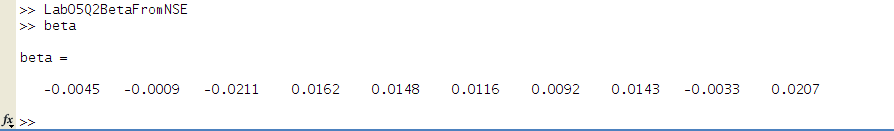
\includegraphics[width=100mm]{BetaNSE}
\end{center}
The $\beta$ values of the stocks included in the index are (in the order as mentioned above) :\\
\begin{center}
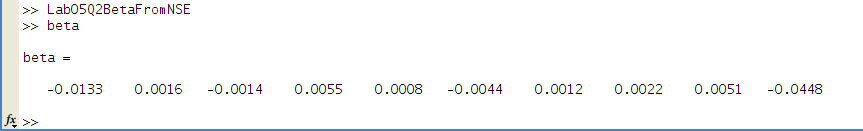
\includegraphics[width=100mm]{BetaStocksIncludedNSE}
\end{center}
Now, the stocks included in the index was used to simulate the index (market portfolio) by taking the weighted average of the prices of the stocks and doing a similar exercise.

The $\beta$ values of the stocks not included in the index obtained by simulating the index from the ten stocks already in the BSE index are (in the order as mentioned above ):\\
\begin{center}
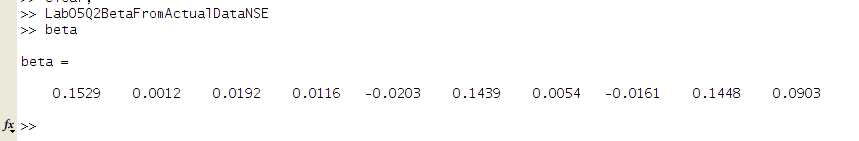
\includegraphics[width=100mm]{BetaActualDataNSE}
\end{center}
--------------------------------------------------------------------------------------

\end{document}